\documentclass[12pt, a4paper]{article}


\usepackage{fancyhdr, enumerate}
\usepackage{amssymb}
\usepackage{geometry, amsmath, amsfonts, float, graphicx}
\usepackage{gensymb}
\usepackage{hyperref, listings}
\usepackage{matlab-prettifier}
\usepackage{caption}
\geometry{
	top=0.9in,           
	inner=0.6in,
	outer=0.6in,
	bottom=2in,
	tmargin= 10ex,       
	headsep=0.6cm,          
}
\pagestyle{fancy}

\fancyhead{}
\fancyfoot{}

\fancyhead[L]{Bioen 316 AC \\Homework 1: Part B\\ April 9, 2019}
\fancyhead[R]{Skyler Hallinan\\ hallisky@uw.edu \\ 1732227}

\lstMakeShortInline[style=Matlab-editor]"
\begin{document}
\vspace*{-3mm}
\section*{Problem}
\begin{enumerate}
\item \begin{enumerate} \item
Go to the \href{http://physionet.org/cgi-bin/atm/ATM}{Physiobank ATM}. Select the PTB Diagnostic ECG Database, and one of the healthy patient records. Download 10 seconds of the signal, starting from anywhere within the signal.  Process the lead I, II, and III columns to have a mean near zero by subtracting the
mean over every half second. Use the lead I and lead II signals, your previous derivation and \textsc{Matlab} to create a
polar plot of the heart axis as it changes over time. 
\item
Use leads I \& III or II \& III to create a new polar plot. Compare the two polar plots
you have created. A large difference is probably a math error, but they might match
well or be a little off. Suggest two reasons why the plots might be slightly different. \end{enumerate}

\item
In the PTB database \href{http://physionet.org/physiobank/database/ptbdb/}{home page},
find the bullets for Input voltage and Resolution. Show that the resolution information
can be used to calculate the input voltage range.
\end{enumerate}

\section*{Solution}


\begin{enumerate}
\item
\begin{enumerate}
\item From the website, we downloaded a two samples of 10 second ecg data: One from a healthy, control patient (patient 104), and one from an unhealthy patient (patient 1). We loaded these into \textsc{Matlab} using "readtable". We then extracted the first three columns of both of these tables, as they corresponded to leads I-III. We converted them to type double for analysis with "cellfun(@str2num,table2array(data)". This gave us two tables of three column data which corresponded to leads I-III for the healthy and unhealthy patients. \\ \\
Our next goal was to set the mean to near zero by subtracting the mean over every half second, using the \textsc{Matlab} function provided, "zeromean.m". For this function, we needed to calculate the sampling rate "fs", where "fs = N/T". Our "T" for both health and unhealthy patients was 10 seconds, and we obtained the number of points in this finite interval "N" by using the "size" command and determining the length of our matrix. We then calculated our "fs" (same for both data) and input our data matrices into the "zeromean" function, along with our calculated "fs". This took each column of the inputted data and made the mean zero. \\ \\
Finally, we calculated the heart vector using the derivations from part A. Using $V_{Hx} = V_I$ and $V_{Hy} = -\frac{1}{\sqrt{3}}({2V_{II} - V_I)}$, we calculated the Cartesian components of the heart vector at each sample. (Note that this $V_{Hy}$ vector is slightly different than in our part A calculations; we forgot to multiply by -1 since the y-component is pointing down). We then converted these coordinates to polar using "cart2pol", and plotted them with "polarplot". We see that our heart vector plot using these I and II leads (Figure 1, left) matches our expectations of a healthy heart.


\begin{figure}[h]
\centering
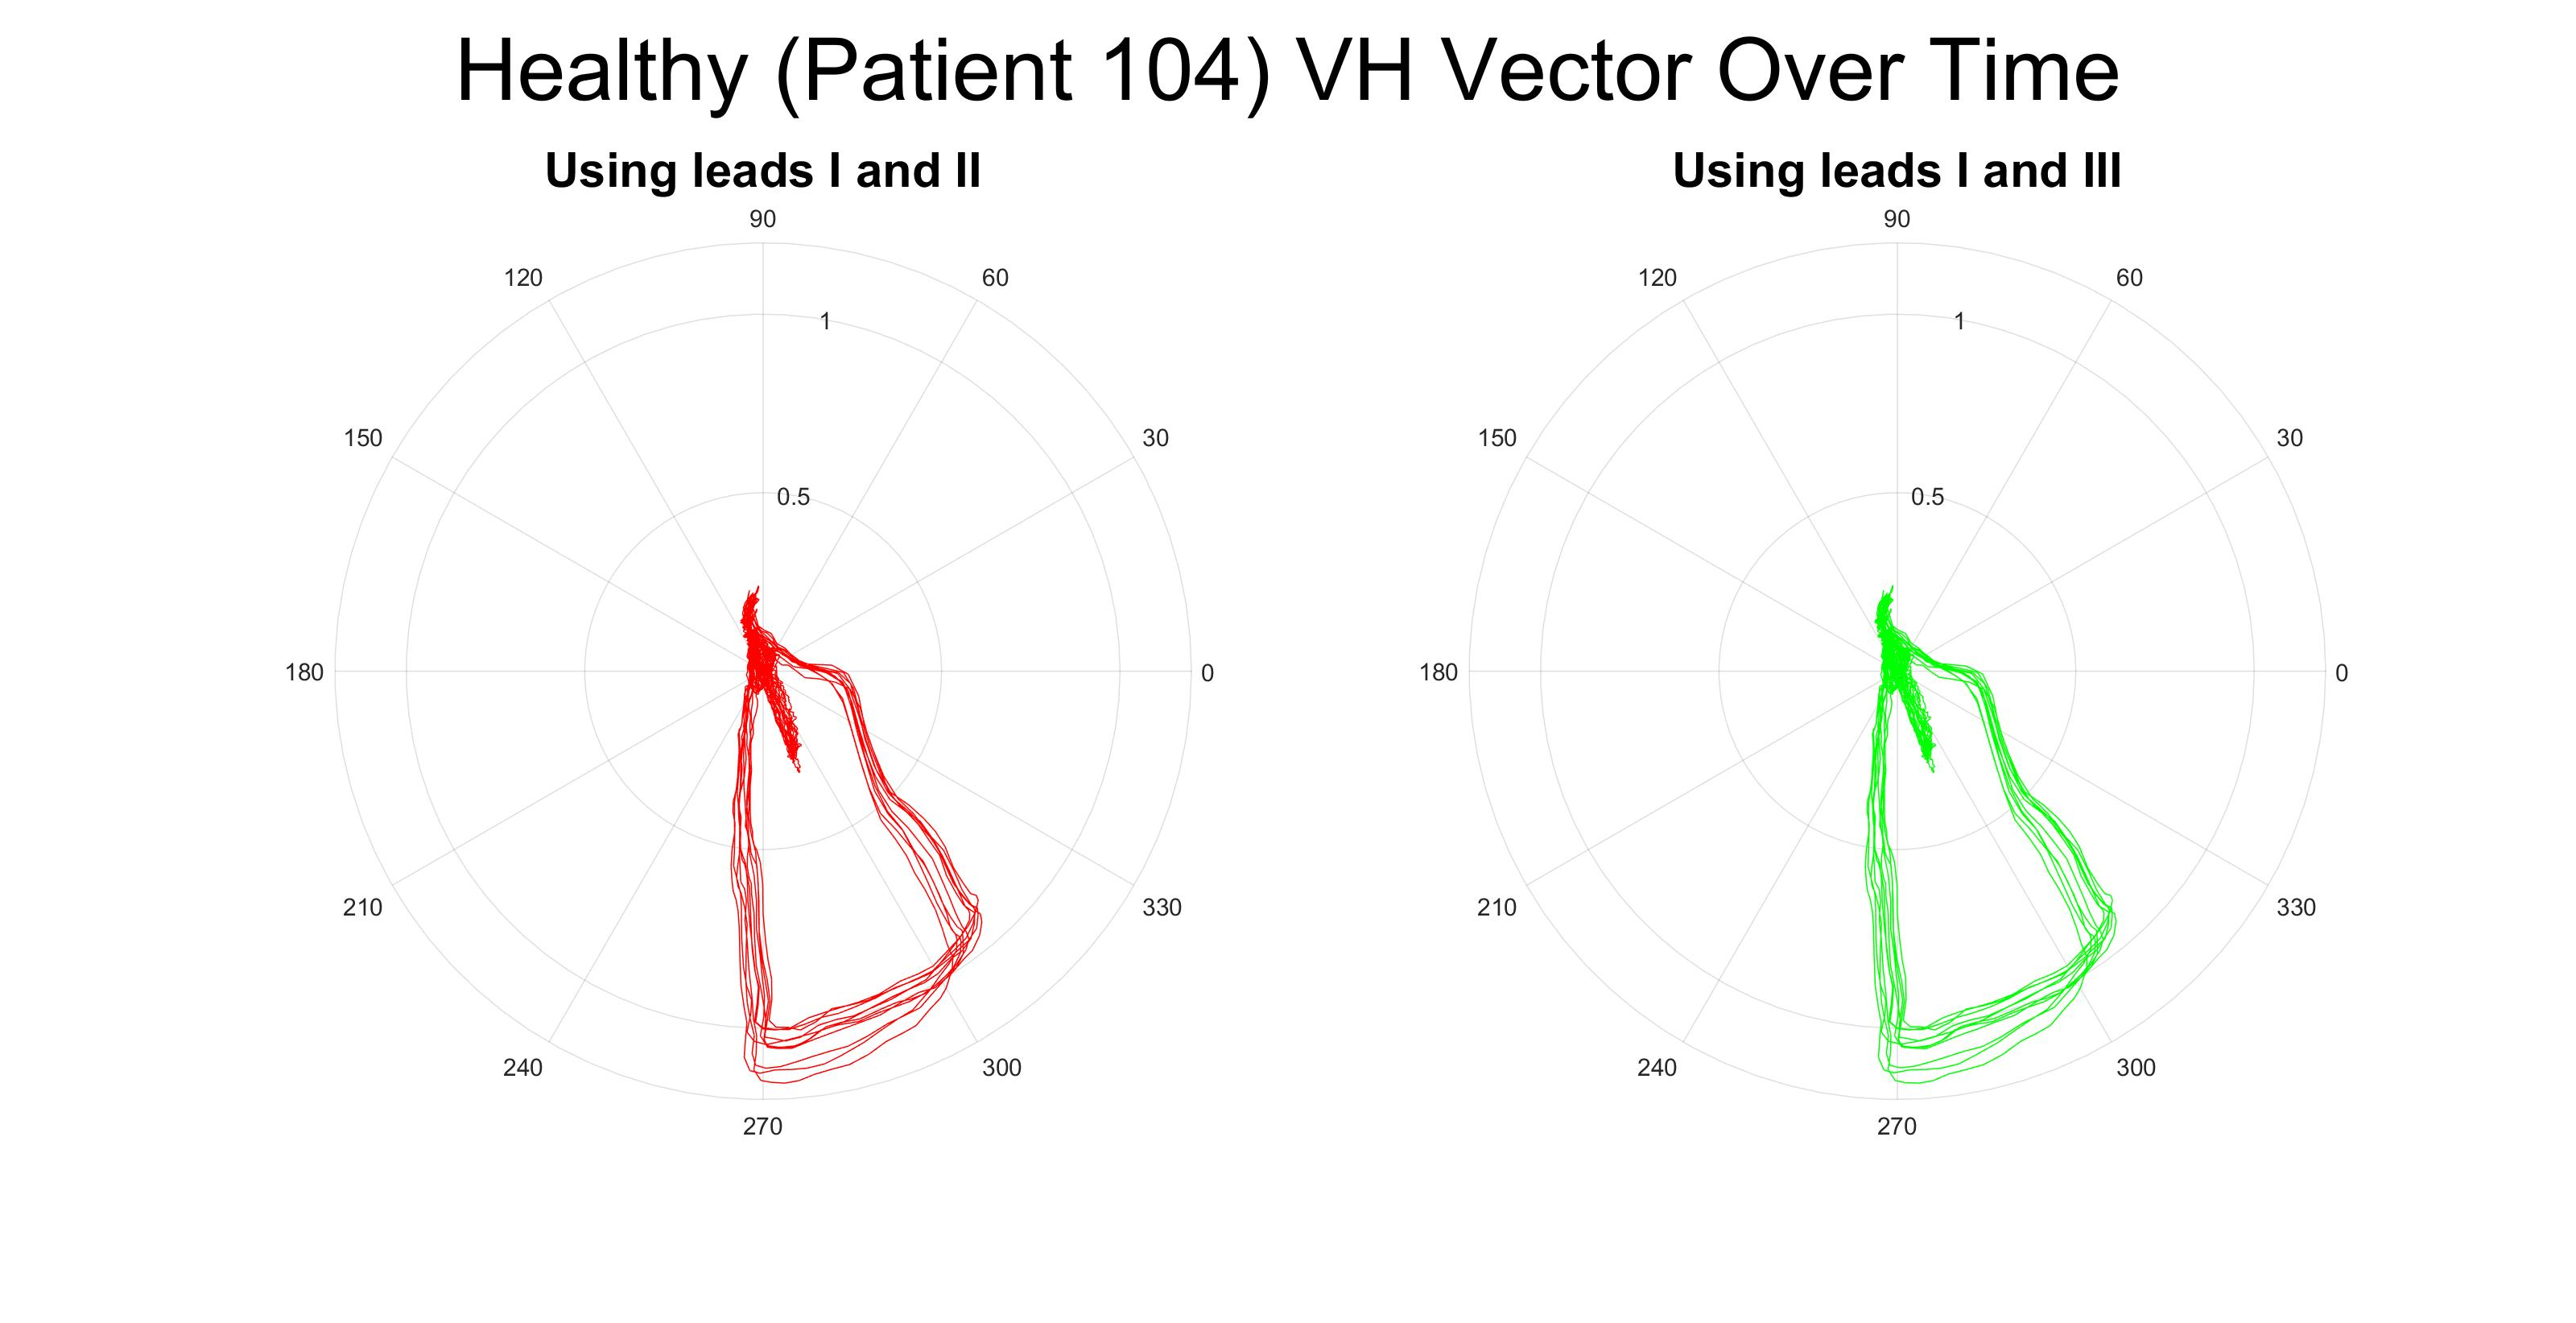
\includegraphics[width=1\textwidth]{ecg1}
\caption{Healthy Patient Heart Vector Derived from Leads I and II (left) and I and III (right)}
\end{figure}


\item 
After making our initial heart vector plot in Figure 1 (left) using leads I and II and our derived formula, we then used leads I and III to calculate the heart vector. As a reminder, Einthoven's Triangle shows the vector relationships between leads I, II, and III. We can use Kirchhoff's rule about the sum of voltages on a closed loop because we are recording voltages around a closed loop with leads I, II, and III. Kirchhoff's rule states that the sum of voltages around a closed loop must be zero: $V_{I} + V_{II} + V_{III} = 0$. \\ \\ 
However, this closed loop rule is the case if all vectors in the loop are head-to-tail with eachother, that is, that the voltage vectors are going in the same direction around the loop. From Einthoven's Triangle, we see that because lead II is going in the opposite direction around the loop, our closed loop rule is $V_{I} - V_{II} + V_{III} = 0 \Rightarrow V_{II} = V_{I} + V_{III}$. \\ \\
\begin{minipage}[t]{\linewidth}
\centering
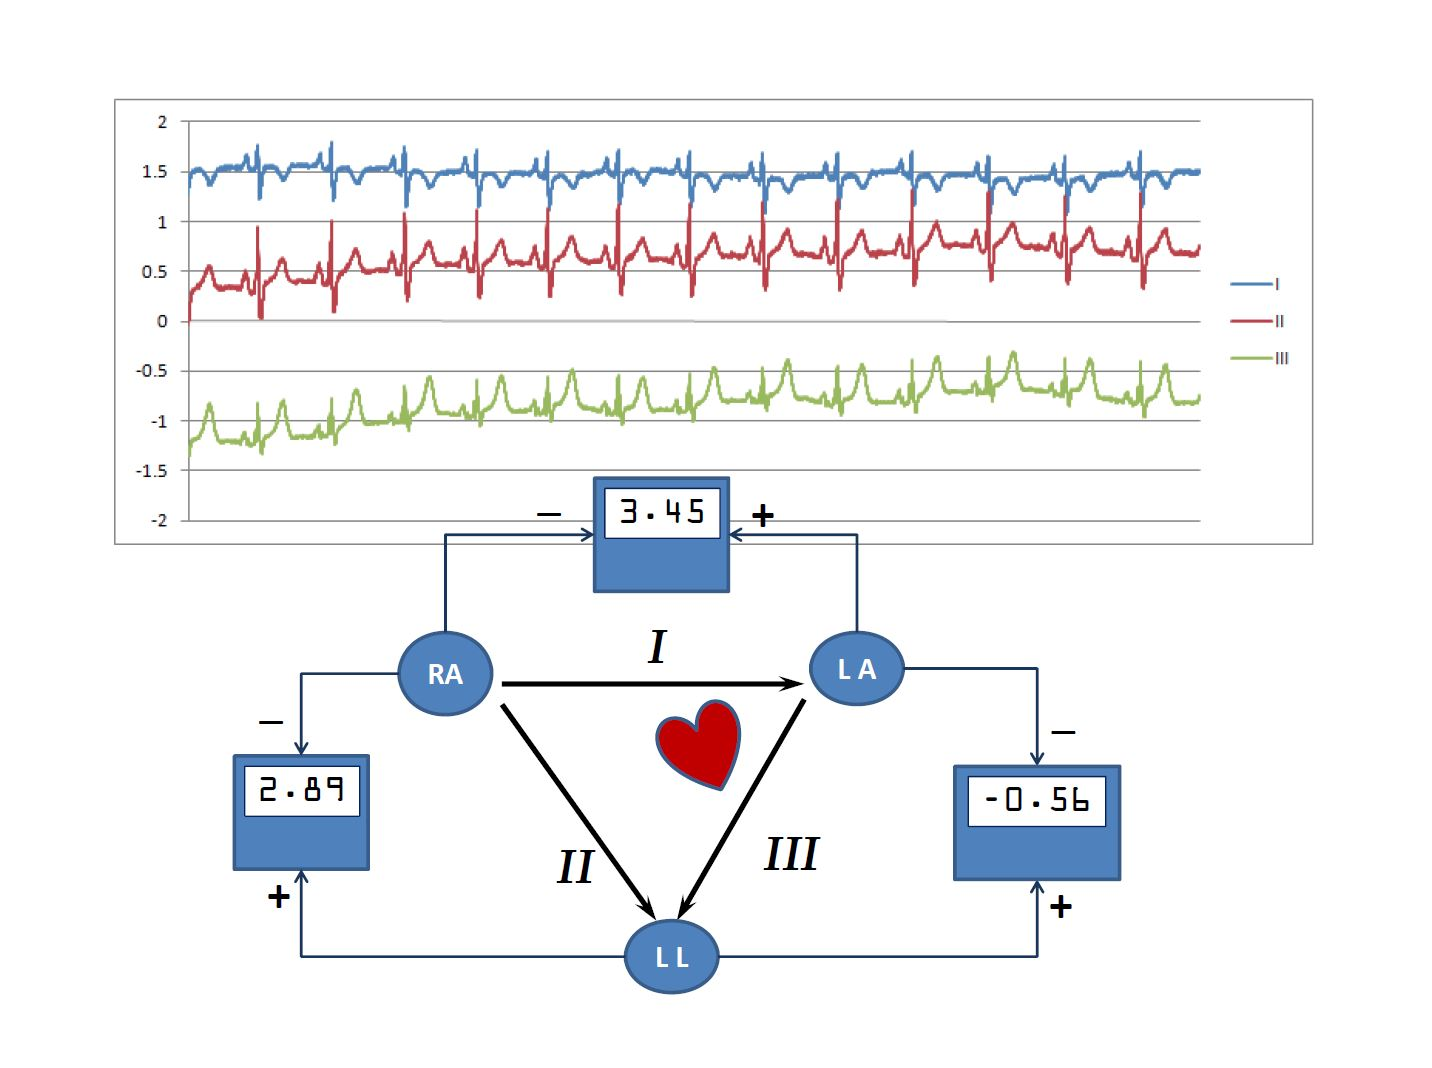
\includegraphics[width=0.6\textwidth]{kirk}
\captionof{figure}{Einthoven's Triangle and Kirchhoff's Rule (from lecture)}
\end{minipage}
\\ \\ \\
In \textsc{Matlab}, to use only leads I and III to calculate the heart vector, we used our same formulas for $V_{Hx}$ and $V_{Hy}$. However, in locations in our derived formula where there was a $V_{II}$ term, we substituted $V_{II} = V_{I} + V_{III}$. This gave us a final output of $V_{Hx} = V_I$ and $V_{Hy} = -\frac{1}{\sqrt{3}}({2(V_{I} + V_{III})- V_I)}$, two equations written in terms of leads I and III. Similar to the previous part, we calculated these Cartesian components, converted to polar, and plotted. \\ \\
We see that in Figure 1, we have near identical plots for our heart vector derived from leads I and II, and derived from I and III. This makes sense; Kirkchoff's rule of a zero voltage around a loop is a universal fact, which makes the substitution we performed logical, and should result in the same polar plot. \\ \\
There are potential reasons for slight differences in the plots, however, which would have made our Kirchhoff's rule substitution less accurate. One reason is that there may have been instrumentation error in the devices used to record the voltages at each of the locations; this may lead to inconsistencies in reading and inaccuracies. Another type of error, a human error, that could have occurred, is that the leads were not placed perfectly in a equilateral triangle with equal angles. Slight deviations from the ideal triangle would make our derived formula slightly inaccurate, as we assumed that the leads were perfectly placed in a equilateral triangle, as shown in Figure 2. Another potential reason for error could be random noise at each of the leads, that varied and was not equal. These leads may have picked up external voltage, noise, at varying levels, which would add to inaccuracies in the data.

\item 
Finally, we made a plot of the unhealthy heart vector over time. We see that this polar plot is very erratic and abnormal compared to a normal control plot. Whereas the healthy vector goes over a controlled path in the bottom right portion of the plot the entire time, the behavior in this is seemingly random and jagged, and is an entirely different location.

\begin{minipage}[t]{\linewidth}
\centering
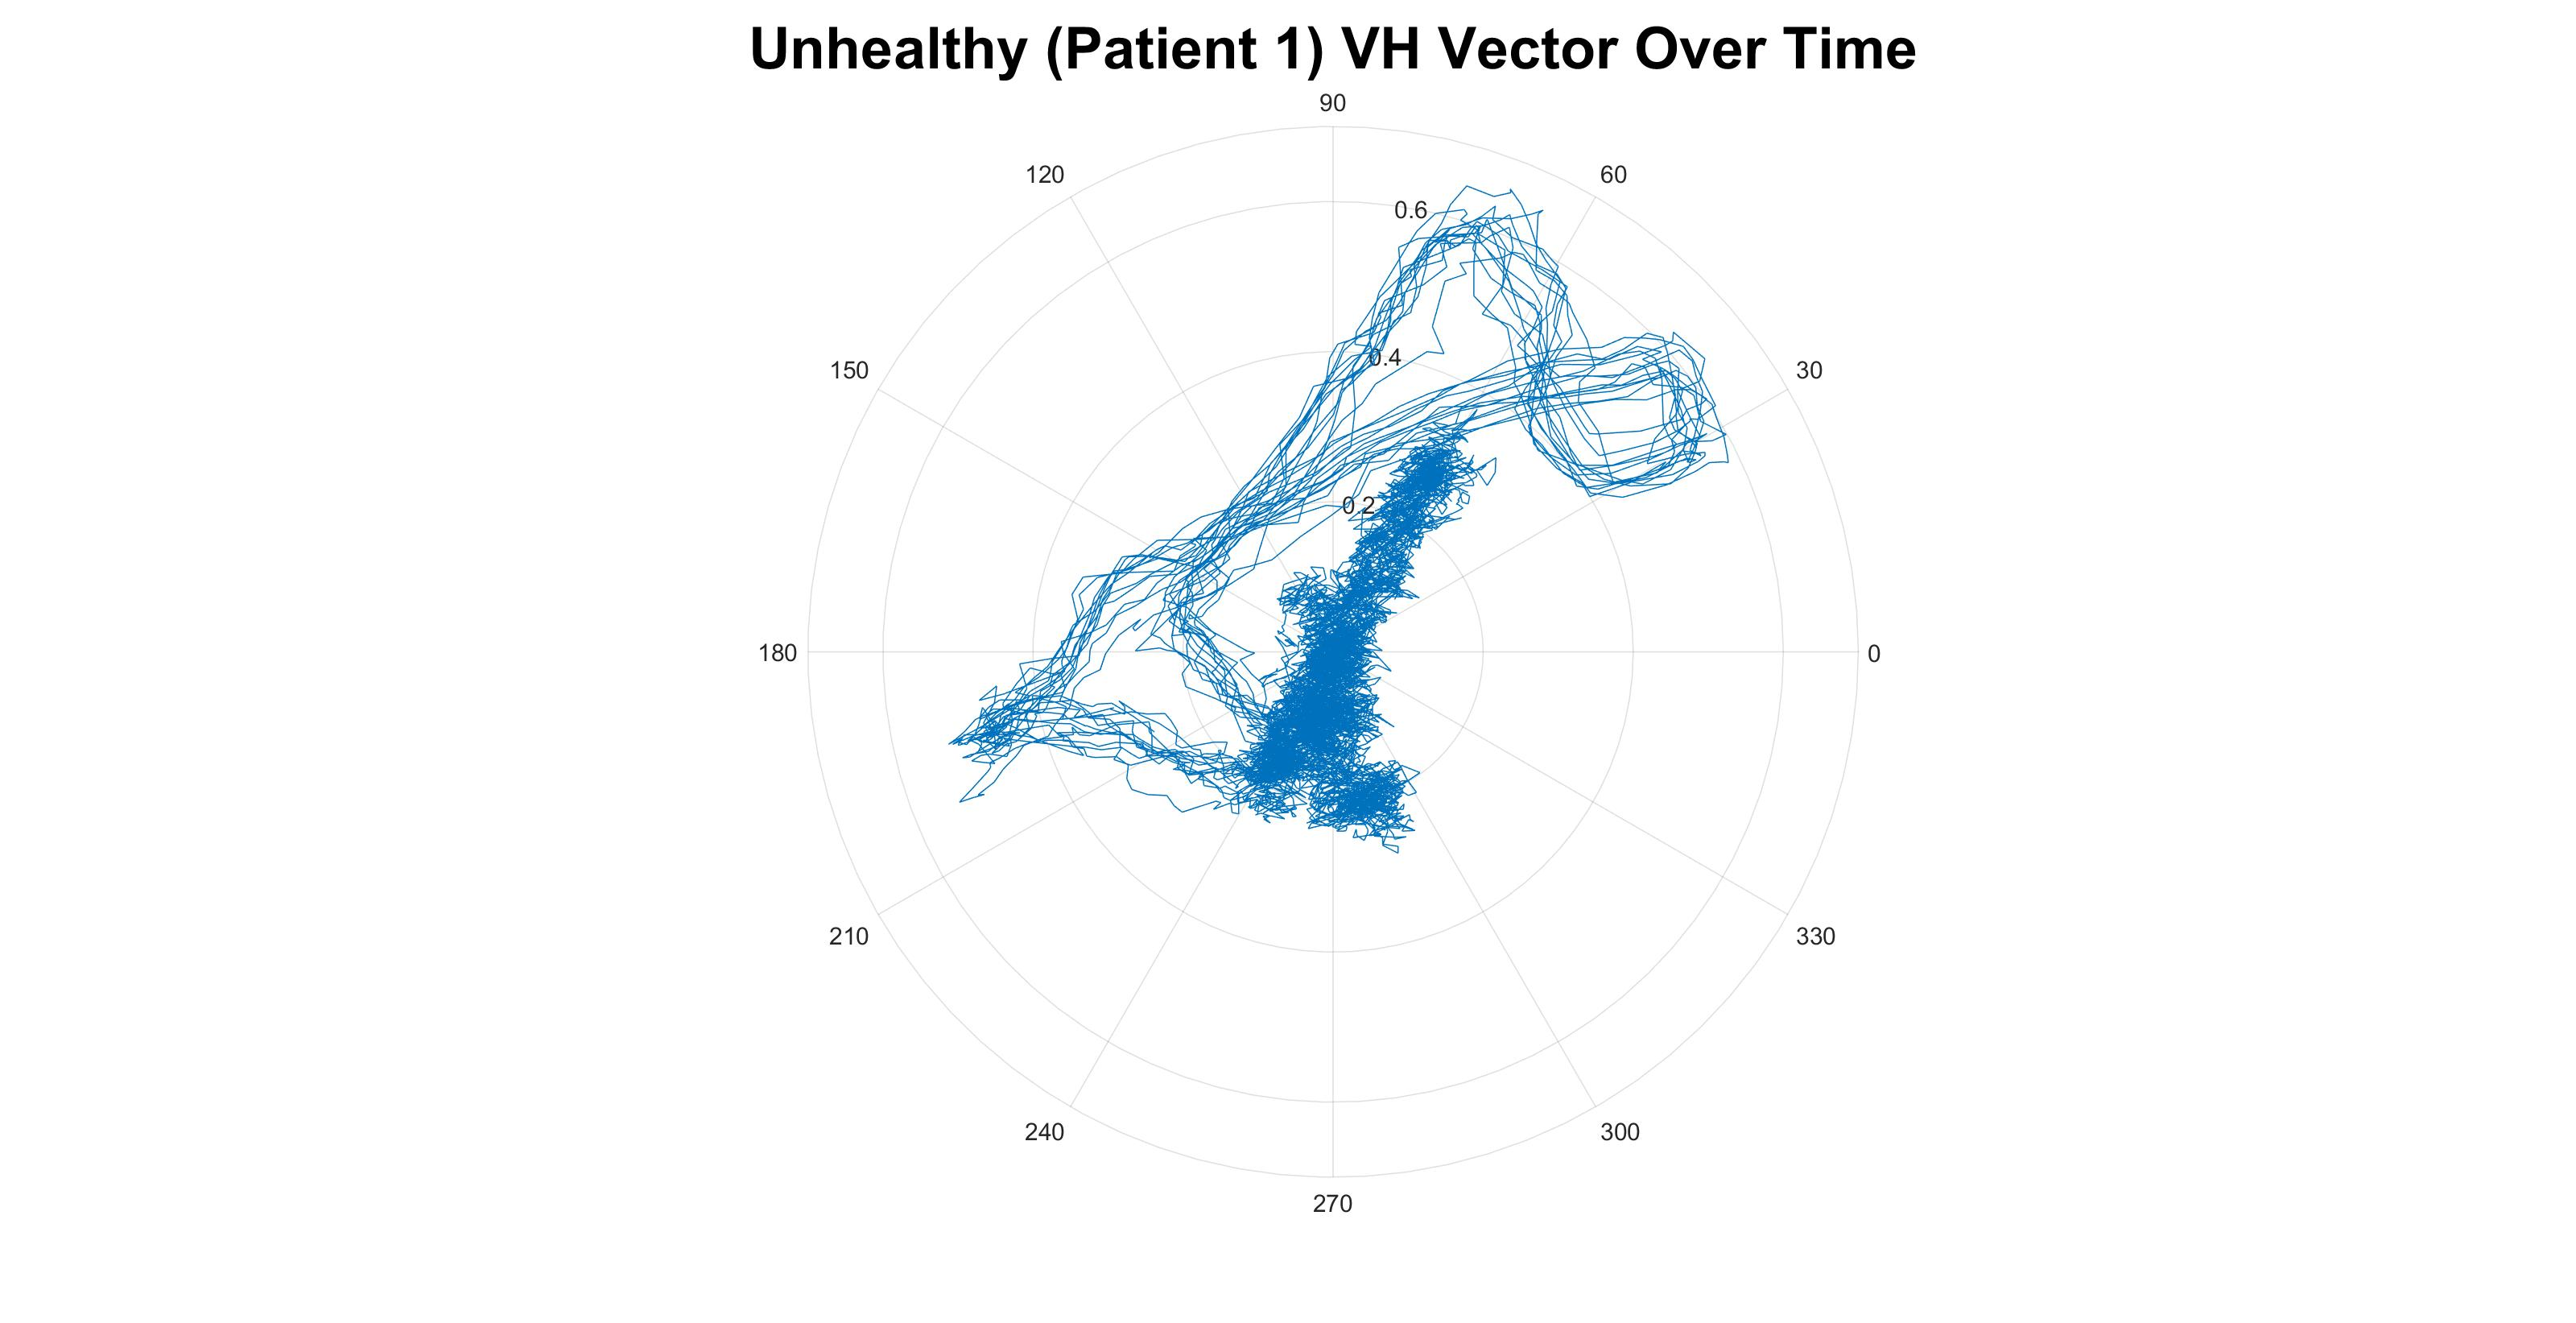
\includegraphics[width=0.6\textwidth]{unhealthyecg}
\captionof{figure}{Unhealthy Heart Vector from Patient 1 (using Leads I and II)}
\end{minipage} \\ \\
\end{enumerate}
\item
 We see that the input voltage is $\pm 16 $ mV, which correponds to an input voltage range of 32 mV. In addition, we see that our resolution is 16 bit with 0.5 $\mu$V/LSB; 16 bits corresponds to $2^{16} = 65536$ unique pieces of information that can be stored as different combinations of the 16 bits. In addition, we see that this resolution tells us our voltage increments represented by going from each bit to the next. \\ \\ 
 We can use the following formula to determine the smallest measurable volage increment represented by the least significant bit: $ q \approx \frac{\Delta V}{2^b}$, where $\Delta V = V_{in, max} - V_{in, min}$, $b$ is the number of bits, and $q$ is the smallest measured voltage increment. We see that $\Delta V = (16 - (-16)) \times 10^{-3} = 32 \times 10^{-3}$, $b = 16$, and $q = 5\times 10^{-7}$. \\ \\
Using this resolution of $5 \times 10^{-7}$ V, we see that we can calculate the input voltage range: \begin{align*}
 q &\approx \frac{\Delta V}{2^b} \\
5 \times 10^{-7} &= \frac{\Delta V}{2^{16}} \\
\Delta V &= 2^{16} \times 5 \times 10^{-7} \\
&= 32.768 \times 10^{-3}
\end{align*}
We see that using our resolution information (number of bits and voltage increments) allows us to calculate the input voltage range with reasonable accuracy. Our calculated voltage range is 32.768 mV, where our actual voltage range is 32 mV. Thus, our calculation is accurate, and we are able to determine the voltage range successfully.

\end{enumerate}
\pagebreak
\section*{\fontsize{19}{15}\selectfont Appendix A}
\subsection*{MATLAB code}
\lstinputlisting[style=Matlab-editor]{hw1.m}
\end{document}